\documentclass{article}
\usepackage{graphicx} % Required for inserting images
\usepackage{float}

\title{apparatus}
\author{Nathan Li}
\date{December 2024}

\begin{document}

\maketitle

\section{Equipment}
    
    \subsection{Laser Source}
        In this experiment, we will use two different laser sources of red light. One is a helium-neon laser with $0.95\,mW$ output power (Figure \ref{laser2}). The other produces red light of wavelength 650 nm with 30 mW output power (Figure \ref{laser2}).

        \begin{figure}[H]
        \centering
        \includegraphics[width=0.5\linewidth]{components/laser 2.jpg}
        \caption{red laser of output power 0.95 mW}
        \label{laser2}
        \end{figure}

         \begin{figure}[H]
        \centering
        \includegraphics[width=0.5\linewidth]{components/laser 1.jpg}
        \caption{red laser of wavelength 650 nm and output power 30 mW}
        \label{laser1}
        \end{figure}

    \subsection{Quantum Design VersaLab}
        The Quantum Design VersaLab (Figure \ref{Versalab}) is a highly automated flexible instrument designed to measure a variety of the physical properties of a sample while controlling the conditions of the sample chamber: temperature (400 to 50 K), magnetic field (up to 3 T), and atmosphere (atmospheric pressure to high vacuum). VersaLab uses a cryocooler to achieve cryogenic temperatures instead of using liquid cryogens.\\
        Also, VersaLab applies a bias current, which is the excitation, to measure the resistance. Versalab will automatically measure the corresponding voltage and then it will give the value of the corresponding resistance based on $R=\frac{V}{I}$. We can also control the limit of the excitation current, voltage, and its power. Also, we can also use constant current mode (current is fixed at the value we set, and voltage and power control is not available). However, unfortunately, VersaLab does not record or show the value of voltage. The most useful things we need from VersaLab are only the values of excitation current and resistance.

        \begin{figure}[H]
        \centering
        \includegraphics[width=0.75\linewidth]{components/VersaLab.png}
        \caption{VersaLab}
        \label{Versalab}
        \end{figure}
        
        In order to observe photoconductivity, we need to use a Type A Multi-Function Probe (MFP, Figure \ref{MFP}) which allows connection between itself and a laser source via a light guide fiber (Figure \ref{fiber}). In addition, an adapter is also needed, and its model will vary due to different fibers that you need to use. So, be sure to get a proper adapter, as it will determine if you can have a good connection between the light source and the MFP.\\
        The MFP is also our sample holder where the sample holder board (Figure \ref{sample holder board}) will be installed.\\
        Based on these features of VersaLab, all we need is just to properly mount our sample on a sample holder board, insert the sample holder board into the MFP, and then plug the MFP into VersaLab.\\

        \begin{figure}[H]
        \centering
        \includegraphics[width=0.5\linewidth]{components/MFP.jpg}
        \caption{Type A Multi-Function Probe (MFP)}
        \label{MFP}
        \end{figure}
        
        \begin{figure}[H]
        \centering
        \includegraphics[width=0.5\linewidth]{components/Fiber-optic cable.jpg}
        \caption{Fiber-optic cable}
        \label{fiber}
        \end{figure}

        \begin{figure}[H]
        \centering
        \includegraphics[width=0.5\linewidth]{components/sample holder board.jpg}
        \caption{Sample holder board}
        \label{sample holder board}
        \end{figure}


    \subsection{MultiVu}
    
        MultiVu is a Windows software that allows us to control the operation of the VersaLab hardware and run the measurements, specifically resistivity.\\
        \begin{figure}[H]
            \centering
            \includegraphics[width=1\linewidth]{main menu.png}
            \caption{main menu of MultiVu}
            \label{main menu}
        \end{figure}
        
        In the main menu, you can see a tool bar at the top and a status bar at the bottom. In the status bar, you need to care mainly about the chamber temperature, magnetic field, chamber pressure (Torr), and sequence status. \\
        In order to change these configurations, click "Instruments" in the tool bar shown in Figure \ref{instrument}.Through here, you are able to change magnetic field, temperature, and chamber pressure (in "Chamber option", you can purge or vent the chamber).\\
        Before you try to put in or take out anything the chamber, you must first make sure that temperature is near 300 K, pressure is near atmospheric pressure, namely 750 Torr, and the magnetic field is 0 T. Keep in mind that always first set the temperature at around 300 K before you vent the chamber (Otherwise, the chamber may be full of ice). If these three conditions are met, you can now start to remove probes in the chamber and install the probe you want to use (Read the Sample Installation section for how to install the MFP).\\
        
        \begin{figure}[H]
            \centering
            \includegraphics[width=0.5\linewidth]{instrument.png}
            \caption{instrument configurations}
            \label{instrument}
        \end{figure}

        After you install the MFP physically, you will also need to install the sample in MultiVu. Click "Utilities" in the tool bar and then click "Activate option" (Figure \ref{utilities}). Then, you will see Figure \ref{activate}. Click "Resistivity" in Available Options and then click "Activate". If you want to deactivate something, just click it in Active Options and then click Deactivate.

        \begin{figure}[H]
            \centering
            \includegraphics[width=0.5\linewidth]{utilities.png}
            \caption{Utilities, where you can activate resistivity measurement option}
            \label{utilities}
        \end{figure}

        \begin{figure}[H]
            \centering
            \includegraphics[width=0.75\linewidth]{activate resis.png}
            \caption{activate resistivity measurement for your sample}
            \label{activate}
        \end{figure}

        After success in activating Resistivity, you should be able to see Figure \ref{install sample}. Now, click "Install/Remove" and then follow the instructions that pop up after you click "Install/Remove". When installing the sample, the Versalab will automatically purge the chamber to around 3 Torr (look at the status bar in Figure \ref{Sample installed and sequence editor}). Notice that the box in front of "Installed" has been checked automatically. If not, you can check the bow manually after recalling if you just install or remove the sample.
        
        \begin{figure}[H]
            \centering
            \includegraphics[width=0.5\linewidth]{install sample.png}
            \caption{Install Sample}
            \label{install sample}
        \end{figure}

        Then, click "Browse" in the Resistivity Option" window (Figure \ref{Sample installed and sequence editor}) and select a file with the extension name .dat or you can create a new one so that data can be properly recorded. By clicking "View", you can see the corresponding data graph as shown in Figure \ref{Data graph}. By right clicking the graph, you are able to change the settings of the graph such as xy axis, log scale, and so on.
        
        \begin{figure}[H]
            \centering
            \includegraphics[width=0.75\linewidth]{sample installed and sequence editor.png}
            \caption{Sample installed and sequence editor}
            \label{Sample installed and sequence editor}
        \end{figure}

        \begin{figure}[H]
            \centering
            \includegraphics[width=0.75\linewidth]{data graph.png}
            \caption{Data graph}
            \label{Data graph}
        \end{figure}

        After sample is installed, activate channels by clicking "Bridge setup". You will see Figure \ref{bridge channel}, and just Check the box of Channel 2 and fill in the blanks of current, power, and voltage limit with 10 as we recommend for most time, and then click set. From now on, you can start to measure the resistance or resistivity. The number you should fill depends on the properties of the sample you are measuring. In general, you need restrict the current, power, and voltage so that the current will not burn your sample. Now, try to click "Measure" in "Resistivity Option" window and then you will see Figure \ref{quick measurement}. Check the box of Channel 2 and fill a number you want in the "Readings". Then, click "Measure" at the bottom left and you can see the resistance of your sample at a certain temperature in a while. This is how you do quick measurement at a certain temperature. For instance, if you want to know the resistance of a $VO_{2}$ film only at 380 K, you set the temperature at 380 K and do such quick measurement. This indeed will save you some time. (See Warnings section for why we use channel 2 here.)
        
        \begin{figure}[H]
            \centering
            \includegraphics[width=1\linewidth]{bridge channels.png}
            \caption{bridge channel}
            \label{bridge channel}
        \end{figure}

        
        \begin{figure}[H]
            \centering
            \includegraphics[width=0.75\linewidth]{quick measure.png}
            \caption{quick measurement}
            \label{quick measurement}
        \end{figure}

        Now, you need a sequence to do an automatic measurement. In tool bar, click "File" and create a new sequence. Then, you should be able to see a selected sequence in the "Selected Sequence" window at the left of the main menu. Then, clicking "Edit", you can see the sequence editor in main menu and the "Sequence Commands" window at the right of main menu, as shown in Figure \ref{Sample installed and sequence editor}. By double clicking commands in the "Sequence Commands" window, you can add commands to the sequence editor. You can follow our sequence or design one on your own based on what you need to do. We set an initial temperature with Fast Settles mode before we start the actual measurements. Notice that there is LogData command in the first line of our sequence, you do not have to add this as well because this is usually useless. But if you use this, please remember that the log data file is different from the file you use to record actual data in "Resistivity Option" window. The LogData will only record the systematic status or so-called diagnostic data. Besides, for the actual measurements, we use Uniform, No O'Shoot mode to scan temperature.\\
        At last, save your sequence file and click Run.\\
    
    \subsection{Sample Installation}
    
            \begin{figure}[H]
                \centering
                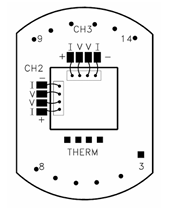
\includegraphics[width=0.25\linewidth]{pin out.png}
                \caption{Pin configuration of resistance bridge sample holder board}
                \label{pin out}
            \end{figure}
            \begin{table}[H]
                \centering
                \begin{tabular}{|c|c|}
                \hline
                   RESISTANCE BRIDGE & RESISTANCE BRIDGE\\
                   BOARD FUNCTION & SAMPLE HOLDER\\
                   \hline
                   Channel 1, I+ & 3    \\  \hline
                   Channel 1, I- & 4    \\  \hline
                   Channel 1, V+ & 5    \\  \hline
                   Channel 1, V- & 6    \\  \hline
                   Channel 2, I+ & 7    \\  \hline
                   Channel 2, I- & 8    \\  \hline
                   Channel 2, V+ & 9    \\  \hline
                   Channel 2, V- & 10   \\  \hline
                   Channel 3, I+ & 11   \\  \hline
                   Channel 3, I- & 12   \\  \hline
                   Channel 3, V+ & 13   \\  \hline
                   Channel 3, V- & 14   \\  \hline
                \end{tabular}
                \caption{Standard interconnection table for sample holder board}
                \label{interconn}
            \end{table}

            First, by looking at the pin configuration (Figure \ref{pin out}), we find that our measurements will be based on 4-terminal measurements. 4-terminal measurement gives more accurate readings since it separates the current carrying wires from voltage sense wires (see more details in section "4-terminal measurements").\\
            
            Before mounting or wiring the sample, please check the interconnection table (Table \ref{interconn}) and pin configuration. We should use \textbf{Channel 3} on the sample holder board, which refers to Pin 11 to 14. (Notice: we need to activate \textbf{Channel 2} in MultiVu later to start the measurement.)\\
            
            After the sample is mounted, we now plug the sample holder board (with sample mounted) to the corresponding part of the MFP (circled in red in Figure \ref{MFP a red}).

            \begin{figure}[H]
                \centering
                \includegraphics[width=0.5\linewidth]{MFP A red.png}
                \caption{Head of a Type A MFP}
                \label{MFP a red}
            \end{figure}

            Then, use puck insertion tool (Figure \ref{puck tool}) to take out the puck inside the VersaLab chamber. The lever of the puck-insertion tool is engaged when it is lying flat across the handle, as is shown in Figure \ref{tool engaged}. When the lever is engaged, the tool grips the puck. Besides, you can also use this tool to install a puck. However, we are not going to use a sample puck in this experiment. You need to use this tool just in case others use a sample puck and leave the puck inside the chamber. A sample puck is a cylinder object as shown in Figure \ref{puck}. It may be either a short or long cylinder.

            \begin{figure}[H]
                \centering
                \includegraphics[width=0.75\linewidth]{components/Puck Insertion Tool .jpg}
                \caption{Puck insertion tool}
                \label{puck tool}
            \end{figure}

            \begin{figure}[H]
                \centering
                \includegraphics[width=0.75\linewidth]{components/puck.png}
                \caption{A sample puck}
                \label{puck}
            \end{figure}

            \begin{figure}[H]
                \centering
                \includegraphics[width=0.25\linewidth]{tool engaged.png}
                \caption{operation of puck insertion tool}
                \label{tool engaged}
            \end{figure}
            
            Now, we install the MFP into the Versalab chamber as shown in Figure \ref{MFP install}. Be sure that you move the MFP smoothly and the O-ring (Figure \ref{O-ring}) sits steadily in the groove on the ferrule of the chamber. Once the MFP reaches the end of the chamber, rotate the MFP slowly until you feel a click. Then, press the MFP a little bit so that the MFP sits steadily in the chamber and can not be rotated any more. Then, attach and tighten the clamp to the ferrule so that the chamber is certainly sealed. If you succeed installing the MFP, you should be able to see Figure \ref{MFP installed}. (Plus: Here we already attached the fiber.)
            
            \begin{figure}[H]
                \centering
                \includegraphics[width=0.75\linewidth, angle=270]{MFP install.jpg}
                \caption{MFP installation}
                \label{MFP install}
            \end{figure}

            \begin{figure}[H]
                \centering
                \includegraphics[width=0.75\linewidth, angle=270]{MFP installed.jpg}
                \caption{MFP installed}
                \label{MFP installed}
            \end{figure}

            \begin{figure}[H]
            \centering
            \includegraphics[width=0.5\linewidth]{components/O ring.jpg}
            \caption{O-ring}
            \label{O-ring}
            \end{figure}

            Now, we need to install the BRT module (Figure \ref{BRT}) which is designated for resistivity measurements.\\
            Look at the panel (Figure \ref{panel}) and find the ports, BRIDGE JL-1 and TEMP JL-3, and then connect the wires of BRT module (Figure \ref{BRT}) to the two ports. Then, connect the BRT module to VersaLab as shown in Figure \ref{BRT install}. Keep in mind that you always align the red dots on BRT module and the panel and that you will not feel resistance if all red dots are aligned when you install the BRT.\\

            \begin{figure}[H]
                \centering
                \includegraphics[width=0.5\linewidth]{components/BRT module.jpg}
                \caption{BRT module}
                \label{BRT}
            \end{figure}

            \begin{figure}[H]
                \centering
                \includegraphics[width=0.75\linewidth]{panel.jpg}
                \caption{Panel on VersaLab}
                \label{panel}
            \end{figure}

            \begin{figure}[H]
                \centering
                \includegraphics[width=0.75\linewidth]{BRT install.jpg}
                \caption{BRT installation}
                \label{BRT install}
            \end{figure}

            Now, it is time to connect the laser source to the MFP by a fiber-optic cable (Figure \ref{fiber}). This is an easy work.\\

            Now, start your measurement on MultiVu.
            
    \subsection{Sample inspection}

    In order to see if your sample is wired correctly, you can use the puck-wiring test station (Figure \ref{station1} and Figure \ref{station2}). You just need to put your sample holder board on the test station and use a digital multimeter to check the resistance between any two of the channels. Also, you can use a magnifier to see how the sample is wired.

        \begin{figure}[H]
        \centering
        \includegraphics[width=0.5\linewidth]{components/Puck-wiring Test Station 1.jpg}
        \caption{puck-wiring test station}
        \label{station1}
        \end{figure}

        \begin{figure}[H]
        \centering
        \includegraphics[width=0.5\linewidth]{components/Puck-wiring Test Station 2.jpg}
        \caption{puck-wiring test station}
        \label{station2}
        \end{figure}

    \subsection{Warnings}
        \subsubsection{Always leave MultiVu open}
            If MultiVu is left closed for more than 5 consecutive minutes, the system automatically shuts down both the magnet and temperature control, so the chamber temperature will start to drift down and usually settles at ~200K if left in that state long enough.
        
        \subsubsection{Procedures to open the chamber}
            1. Set the chamber temperature at 300 K.\\
            2. After the temperature is steady around 300 K, vent the chamber.\\
            3. Set the magnetic field at 0 T.\\
            4. Deactivate the measurement option that you are using now.\\
            5. Take whatever inside the chamber out.\\
        \textbf{Always follow these steps. Otherwise, the chamber might be frozen.}\\

        \subsubsection{Do not tighten the clamp too much when you insert the MFP into the chamber}

        \subsubsection{BRT module redirects the channels of the sample holder board}
            If you wire the sample on channel 2 (respectively, 3) of the sample holder board, you should use channel 1 (respectively, 2) on MultiVu. So, be careful which channel you are using and do not use the wrong channel.
    

\end{document}
